\section{Workspace for Model-to-Text Transformation}

- Start Eclipse with empty Workspace
- Switch to the moflon perspective

%\usepackage{graphics} is needed for \includegraphics
\begin{figure}[!htbp]
\begin{center}
 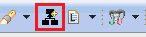
\includegraphics[width=0.3\textwidth]{pics/moca/1DictionaryMetaModel/1-NewMetamodelWizard}
  \caption{Opening the ``New Metamodel'' wizard}
  \label{moca-1-NewMetamodelWizard}
\end{center}
\end{figure}

- Open the ``New Metamodel'' wizard 

%\usepackage{graphics} is needed for \includegraphics
\begin{figure}[!htbp]
\begin{center}
 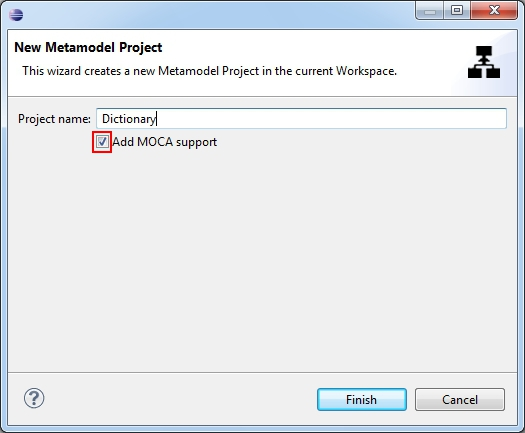
\includegraphics[width=0.7\textwidth]{pics/moca/1DictionaryMetaModel/2-AddMocaSupport-ProjectName}
  \caption{Add Metamodel project with MOCA support}
  \label{moca-2-AddMocaSupport-ProjectName}
\end{center}
\end{figure}

- Set project name to ``Dictionary''
- Select "Add Moca Support" 


%\usepackage{graphics} is needed for \includegraphics
\begin{figure}[!htbp]
\begin{center}
 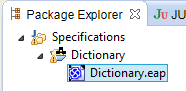
\includegraphics[width=0.3\textwidth]{pics/moca/1DictionaryMetaModel/3-WizardResult}
  \caption{Workspace after wizard finishes}
  \label{moca-3-WizardResult}
\end{center}
\end{figure}

- Project and eap file are created (see Fig. \ref{moca-3-WizardResult})

%\usepackage{graphics} is needed for \includegraphics
\begin{figure}[!htbp]
\begin{center}
 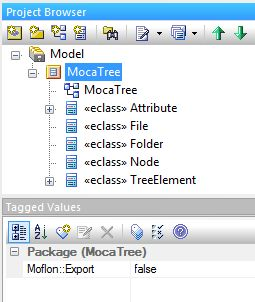
\includegraphics[width=0.5\textwidth]{pics/moca/1DictionaryMetaModel/4-eapContainsMocatreeWithExportFalse}
  \caption{The EA project contains a package ``MocaTree'' with property
  $Moflon::Export = false$}
  \label{moca-4-eapContainsMocatreeWithExportFalse}
\end{center}
\end{figure}

- open Dictionary.eap
- eap file contains MocaTree package with $export = false$ (Fig.
\ref{moca-4-eapContainsMocatreeWithExportFalse})

\begin{figure}[!htbp]
\begin{center}
 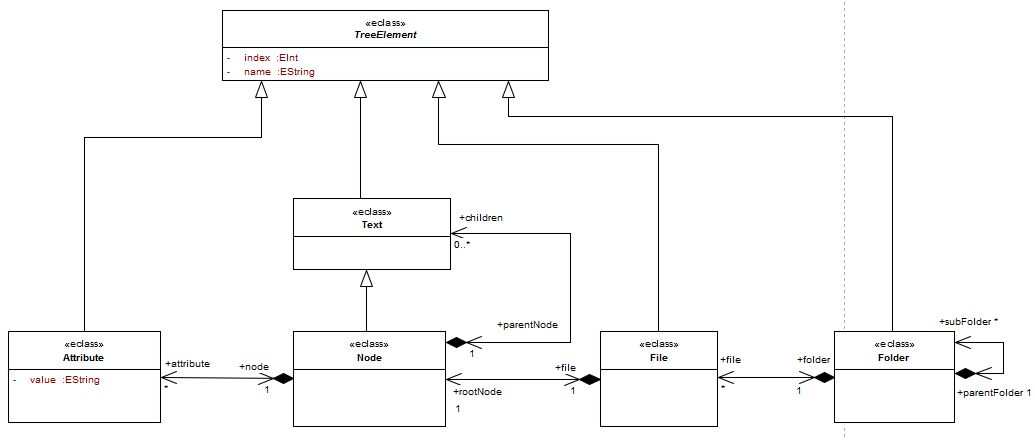
\includegraphics[width=\textwidth]{pics/moca/0Install/0-MocaTree}
  \caption{Mocatree metamodel}
  \label{moca-tree}
\end{center}
\end{figure}
 

%\usepackage{graphics} is needed for \includegraphics
\begin{figure}[!htbp]
\begin{center}
 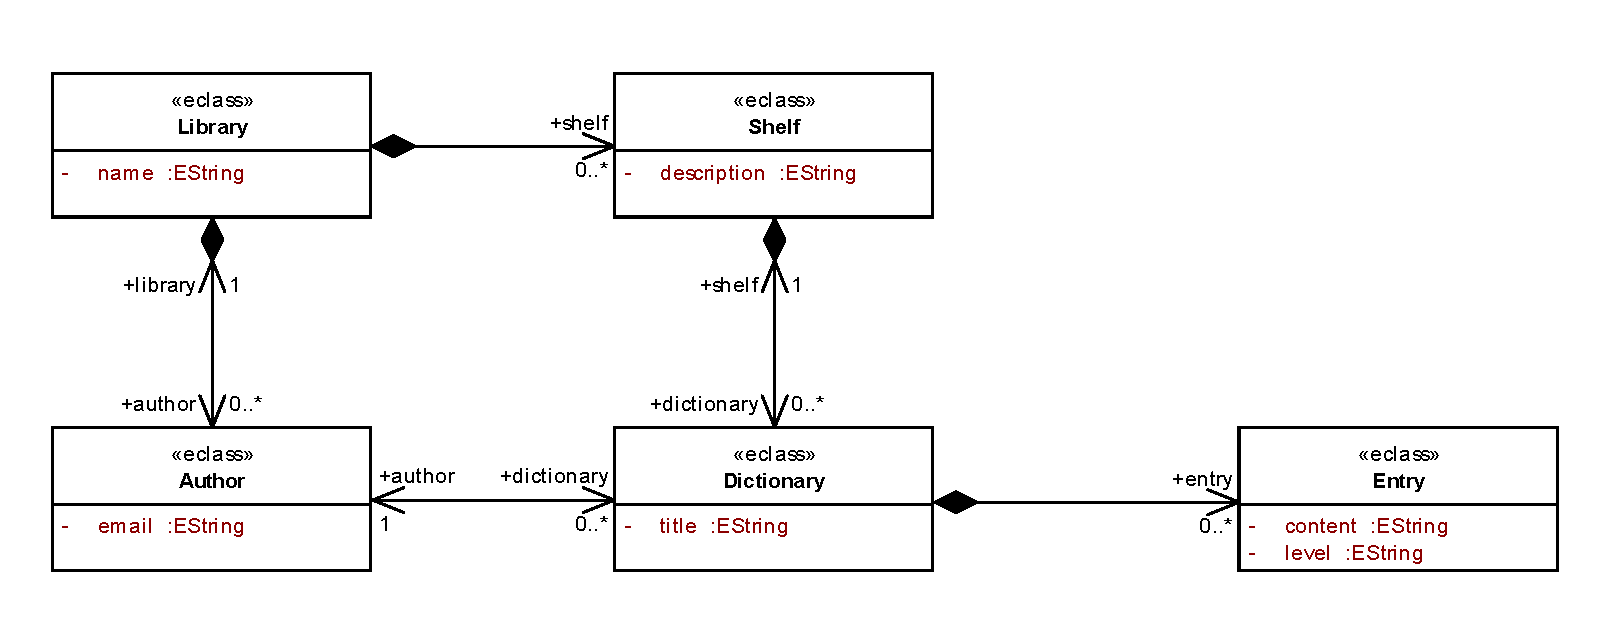
\includegraphics[width=\textwidth]{pics/moca/1DictionaryMetaModel/DictionaryLanguage}
  \caption{Dictionary metamodel}
  \label{moca-5-DictionaryMM}
\end{center}
\end{figure}

- Add dictionary Metamodel like in (Fig. \ref{moca-5-DictionaryMM})
- Add package ``DictionaryCodeAdapter''

%\usepackage{graphics} is needed for \includegraphics
\begin{figure}[!htbp]
\begin{center}
 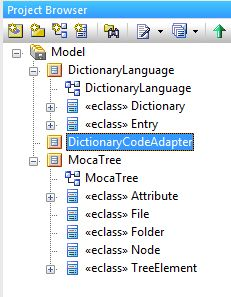
\includegraphics[width=0.5\textwidth]{pics/moca/1DictionaryMetaModel/5-DictionaryMM-ProjectBrowser}
  \caption{EA project view before exporting}
  \label{moca-5-DictionaryMM-ProjectBrowser}
\end{center}
\end{figure}

- EA projects just before export (Fig. \ref{moca-5-DictionaryMM-ProjectBrowser}) 

%\usepackage{graphics} is needed for \includegraphics
\begin{figure}[!htbp]
\begin{center}
 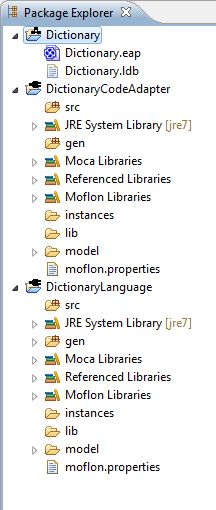
\includegraphics[width=0.3\textwidth]{pics/moca/1DictionaryMetaModel/6-ExportToEclipse}
  \caption{Workspace after export to eclipse}
  \label{moca-6-ExportToEclipse}
\end{center}
\end{figure}

- Export to eclipse  (Fig. \ref{moca-6-ExportToEclipse})
